\documentclass[aspectratio=169, table]{beamer}

\usepackage{array}
\usepackage{colortbl}
\usepackage{tabularx}
\usepackage{xcolor}
\usepackage{tikz}
\usetikzlibrary{arrows.meta, positioning, calc, fit}

\makeatletter
\def\input@path{{../theme/}}
\makeatother
\graphicspath{{../theme/}{../../figures/}}
\usetheme{Pradita}

\newcommand{\sectionframe}[1]{%
  \begin{frame}{\hfill}
    \centering
    \Huge{\textbf{#1}}
  \end{frame}
}

\newcommand{\takeaway}[1]{%
  \vspace{4pt}
  {\footnotesize #1}
}

\title{\huge Lapisan Motivasi:\\
  \vspace{8pt}
  API Transfer Dana}
\subtitle{IT30713 - Enterprise \& Platform Architecture}
\author{\textbf{Alfa Yohannis}}
\date{6 Juni 2026}

\begin{document}

\frame{\titlepage}

\begin{frame}[fragile]
  \frametitle{Contents}
  \vspace{20pt}
  \begin{columns}[t]
    \column{0.5\textwidth}
    \tableofcontents[sections={1-4}]

    \column{0.5\textwidth}
    \tableofcontents[sections={5-8}]
  \end{columns}
\end{frame}

\begin{frame}{\hfill}
  \centering
  \Huge{\textbf{Mengapa perusahaan perlu menambahkan kapabilitas?}}
\end{frame}

% ============================================================
\section{Orientasi Bab}
\sectionframe{Orientasi Bab}

\begin{frame}{Tujuan Pembelajaran}
  \vspace{8pt}
  \begin{itemize}
    \item Menjelaskan elemen \textbf{lapisan motivasi} ArchiMate: pemangku
          kepentingan, pendorong, asesmen, sasaran, hasil, kebutuhan, kendala,
          prinsip, makna, dan nilai.
    \item Menyusun \textbf{model motivasi} untuk satu kapabilitas sasaran:
          API (\emph{Application Programming Interface}) Transfer dan Perpindahan Dana Bank Wanua.
    \item Mengidentifikasi \textbf{ketidakselarasan} antara sasaran dan kondisi
          nyata sebagai sumber masalah penelitian.
    \item Merumuskan \textbf{rumusan masalah, RQ (pertanyaan penelitian), dan kontribusi} awal yang
          berakar pada lapisan motivasi.
  \end{itemize}
  \takeaway{Arah sesi: dari ``mengapa'' menuju masalah penelitian yang tajam.}
\end{frame}

\begin{frame}{Ringkasan Awal Bab}
  \vspace{6pt}
  \begin{itemize}
    \item Lapisan motivasi menjawab \emph{mengapa} arsitektur dibangun---sebelum
          \emph{apa} dan \emph{bagaimana}.
    \item Studi kasus berjalan: \textbf{API Transfer dan Perpindahan Dana} Bank
          Wanua---``rel'' (\emph{payment rails}: fondasi perpindahan dana) yang membungkus BI-FAST (\emph{Bank Indonesia Fast Payment}) dan transaksi antarrekening.
    \item Keluaran bab memperkuat \textbf{Pendahuluan} makalah: latar belakang,
          RQ, dan kontribusi awal.
  \end{itemize}
  \takeaway{Motivasi yang jelas membuat rekomendasi teknologi dapat ditelusuri
  kembali ke alasan bisnis.}
\end{frame}

% ============================================================
\section{Mengapa Lapisan Motivasi}
\sectionframe{Mengapa Lapisan Motivasi}

\begin{frame}{Dari ``Mengapa'' ke ``Apa'' dan ``Bagaimana''}
  \vspace{6pt}
  \begin{itemize}
    \item Banyak inisiatif digital gagal bukan karena teknologi lemah, tetapi
          karena tidak jelas \emph{siapa dilayani}, \emph{pendorong} mana yang
          mendesak, dan \emph{sasaran} apa yang dikejar.
    \item ``Membuka API'' tanpa pemangku kepentingan yang jelas, atau
          ``transfer real-time'' tanpa menyatakan kendala regulasi dan sistem
          lama, adalah resep ketidakselarasan.
  \end{itemize}
  \takeaway{Bagi pembaca non-IT: keputusan arsitektur pada dasarnya keputusan
  manajerial---pelanggan, anggaran, regulasi, risiko, reputasi.}
\end{frame}

% ============================================================
\section{Kerangka: TOGAF ADM dan Lapisan ArchiMate}
\sectionframe{Kerangka: TOGAF ADM dan Lapisan ArchiMate}

\begin{frame}{Siklus TOGAF ADM}
  \vspace{15pt}
  \begin{columns}[c]
    \column{0.4\textwidth}
    \centering
    \scalebox{0.85}{
      \begin{tikzpicture}[
        font=\footnotesize\bfseries,
        phase/.style={circle, draw=praditagreen, line width=0.4mm,
          fill=praditagreen!15, minimum size=11mm, inner sep=0pt},
        reqman/.style={circle, draw=blueColor, line width=0.4mm, fill=blueColor!15,
          minimum size=21mm, inner sep=1pt, align=center, font=\scriptsize\bfseries},
        prelim/.style={circle, draw=orange!80!black, line width=0.4mm,
          fill=orange!25, minimum size=13mm, inner sep=0pt, align=center,
          font=\scriptsize\bfseries},
        ring/.style={-Latex, draw=praditagreen!75, line width=0.4mm},
        spoke/.style={draw=blueColor!35, line width=0.25mm},
      ]
        \node[reqman] (rm) at (0,0) {Manajemen\\Requirements};
        \foreach \ang/\lab in {90/A, 45/B, 0/C, -45/D, -90/E, -135/F, 180/G, 135/H}
          \node[phase] (\lab) at (\ang:2.6cm) {\lab};
        \node[prelim] (P) at (90:4.1cm) {Prelim.};
        \foreach \lab in {A,B,C,D,E,F,G,H} \draw[spoke] (\lab) -- (rm);
        \foreach \a/\b in {A/B, B/C, C/D, D/E, E/F, F/G, G/H, H/A}
          \draw[ring] (\a) to[bend left=12] (\b);
        \draw[ring, draw=orange!80!black] (P) -- (A);
      \end{tikzpicture}
    }
    \column{0.6\textwidth}
    {\footnotesize TOGAF (\emph{The Open Group Architecture Framework}); ADM
    (\emph{Architecture Development Method})---metode pengembangan arsitektur
    dengan siklus berulang.\par}
    \vspace{5pt}
    \footnotesize
    \begin{itemize}\setlength{\itemsep}{1.0pt}
      \item \textbf{Prelim.}---Persiapan \& prinsip
      \item \textbf{A}---Visi Arsitektur
      \item \textbf{B}---Arsitektur Bisnis
      \item \textbf{C}---Arsitektur Sistem Informasi (Data \& Aplikasi)
      \item \textbf{D}---Arsitektur Teknologi
      \item \textbf{E}---Peluang \& Solusi
      \item \textbf{F}---Perencanaan Migrasi
      \item \textbf{G}---Tata Kelola Implementasi
      \item \textbf{H}---Manajemen Perubahan Arsitektur
      \item \textbf{Manajemen Requirements}---di pusat, menautkan dan
    menyetir semua fase
    \end{itemize}
  \end{columns}
\end{frame}

\begin{frame}{Fase \emph{Preliminary}}
  \vspace{2pt}
  \footnotesize
  \begin{columns}[t]
    \column{0.5\textwidth}
    \textbf{Apa \& Mengapa}
    \begin{itemize}\setlength{\itemsep}{2.5pt}
      \item Fase \emph{persiapan} sebelum siklus ADM---menata organisasi,
            lingkup, prinsip, tim, dan tata kelola arsitektur.
      \item Menjawab \emph{di mana, apa, mengapa, siapa, bagaimana} arsitektur
            dikerjakan di perusahaan ini.
      \item Memperkirakan \emph{waktu, biaya, dan risiko} memadai secara garis besar.
      \item Mengamankan komitmen pimpinan sebelum biaya besar dikeluarkan.
    \end{itemize}

    \column{0.5\textwidth}
    \textbf{Bagaimana}
    \begin{enumerate}\setlength{\itemsep}{2.5pt}
      \item Tetapkan \textbf{ruang lingkup}: unit dan kapabilitas terdampak.
      \item Bentuk \textbf{tim arsitektur} beserta peran dan mandat.
      \item Rumuskan \textbf{prinsip} (patuh dahulu, penggunaan ulang,
            \emph{API-first}).
      \item \textbf{Sesuaikan kerangka} dan \textbf{pilih alat} (ArchiMate +
            Archi).
      \item Siapkan \textbf{repositori dan tata kelola} awal.
    \end{enumerate}
  \end{columns}
  \vspace{2pt}
  \takeaway{\textbf{Bank Wanua:} lingkup = API Transfer Dana; prinsip = patuh
  SNAP BI (Standar Nasional Open API Pembayaran), bungkus BI-FAST, kendali
  biaya; alat = ArchiMate di Archi.}
\end{frame}

\begin{frame}{Visi Arsitektur (Fase A)}
  \vspace{2pt}
  \footnotesize
  \begin{columns}[t]
    \column{0.5\textwidth}
    \textbf{Apa \& Mengapa}
    \begin{itemize}\setlength{\itemsep}{2.5pt}
      \item Langkah \emph{pertama} siklus: \emph{gambaran tingkat tinggi} arah,
            nilai, dan kapabilitas yang dituju.
      \item Tetapkan lingkup, pemangku kepentingan, sasaran, ukuran
            keberhasilan; disahkan lewat \emph{Statement of Architecture Work}.
      \item Menyatukan persepsi ``mau ke mana dan mengapa layak'' sebelum
            kerja rinci dan investasi besar.
      \item Mengamankan dukungan dan mandat; membatasi lingkup agar realistis.
    \end{itemize}

    \column{0.5\textwidth}
    \textbf{Bagaimana}
    \begin{enumerate}\setlength{\itemsep}{2.5pt}
      \item Identifikasi \textbf{pemangku kepentingan} dan \emph{concern}.
      \item Tegaskan \textbf{pendorong, sasaran, dan kendala}.
      \item Sketsa \textbf{baseline vs.\ target} tingkat tinggi.
      \item Tetapkan \textbf{lingkup}, \textbf{KPI} (Indikator Kinerja Utama),
            dan risiko.
      \item Susun \textbf{Visi} dan \emph{Statement of Architecture Work} untuk
            disahkan.
    \end{enumerate}
  \end{columns}
  \vspace{2pt}
  \takeaway{Di sinilah \textbf{lapisan motivasi} dibangun (pemangku
  kepentingan, pendorong, asesmen, sasaran)---bahan langsung model motivasi
  sesi ini.}
\end{frame}

\begin{frame}{Lapisan dan Aspek ArchiMate}
  \vspace{2pt}
  \centering
  \scalebox{0.78}{
    \begin{tikzpicture}[
      font=\small\bfseries,
      node distance=2.2mm,
      layer/.style={draw, rounded corners=1.5mm, align=left, minimum width=82mm,
        minimum height=10mm, inner xsep=4mm},
      strat/.style={layer, fill=purple!16},
      biz/.style={layer, fill=praditagreen!22},
      app/.style={layer, fill=blue!14},
      tech/.style={layer, fill=gray!18},
      impl/.style={layer, fill=orange!20},
    ]
      \node[strat] (s) {STRATEGI\\
        \footnotesize\mdseries Sumber daya, kapabilitas, arah tindakan};
      \node[biz, below=of s] (b) {BISNIS\\
        \footnotesize\mdseries Aktor, peran, proses, dan layanan bisnis};
      \node[app, below=of b] (a) {APLIKASI\\
        \footnotesize\mdseries Komponen, layanan, dan antarmuka aplikasi};
      \node[tech, below=of a] (t) {TEKNOLOGI (\& FISIK)\\
        \footnotesize\mdseries Node, perangkat, jaringan, \emph{system software}};
      \node[impl, below=of t] (i) {IMPLEMENTASI \& MIGRASI\\
        \footnotesize\mdseries \emph{Work package}, \emph{deliverable},
        \emph{plateau}, \emph{gap}};
      \node[draw, rounded corners=2mm, fill=purple!28, align=center,
        text width=16mm, minimum height=60mm, right=5mm of a, font=\bfseries]
        (mot) {M\\O\\T\\I\\V\\A\\S\\I\\[2mm]\footnotesize\mdseries (mengapa)};
    \end{tikzpicture}
  }
  \takeaway{Tiga lapisan inti---Bisnis, Aplikasi, Teknologi. Aspek
  \textbf{Motivasi} (``mengapa'') melingkupi semua lapisan: fokus sesi ini.}
\end{frame}

\begin{frame}{Pemetaan Lapisan ke Fase ADM}
  \vspace{2pt}
  \scriptsize
  \setlength{\extrarowheight}{2pt}
  \arrayrulecolor{black!65}\setlength{\arrayrulewidth}{0.4pt}
  \begin{tabularx}{\textwidth}{|p{0.30\textwidth}|X|}
    \hline
    \rowcolor{praditagreen!18}
    \textbf{Lapisan / Aspek ArchiMate} & \textbf{Fase TOGAF ADM Terkait} \\
    \hline
    Motivasi (aspek) & Preliminary, A (Visi Arsitektur) \\
    \hline
    Strategi & A -- Visi Arsitektur \\
    \hline
    Bisnis & B -- Arsitektur Bisnis \\
    \hline
    Aplikasi & C -- Arsitektur Sistem Informasi (Aplikasi) \\
    \hline
    Data / Informasi & C -- Arsitektur Sistem Informasi (Data) \\
    \hline
    Teknologi (\& Fisik) & D -- Arsitektur Teknologi \\
    \hline
    Implementasi \& Migrasi & E, F -- Peluang \& Solusi, Perencanaan Migrasi \\
    \hline
  \end{tabularx}

  \vspace{4pt}
  \takeaway{Lapisan motivasi terutama dibangun di fase \emph{Preliminary} dan
  \textbf{A (Visi)}, lalu dipelihara melalui Manajemen Persyaratan.}
\end{frame}

\begin{frame}{Business Model Canvas (BMC)}
  \vspace{20pt}
  {\footnotesize Satu lembar untuk memetakan
  \emph{bagaimana} organisasi menciptakan, memberikan, dan menangkap
  nilai---sembilan blok bangunan.\par}
  \vspace{4pt}
  \centering
  \resizebox{\textwidth}{!}{
    \begin{tikzpicture}[
      font=\scriptsize,
      box/.style={draw=black!55, line width=0.3pt, inner sep=3pt, anchor=center,
        align=center},
    ]
      \node[box, minimum width=2.4cm, minimum height=3.2cm, fill=blue!10,
        text width=2.15cm] at (1.2,2.9)
        {\textbf{Kemitraan Utama}\\{\tiny\itshape Key Partners}\\[3pt]
         {\tiny Mitra \& pemasok kunci}};
      \node[box, minimum width=2.4cm, minimum height=1.6cm, fill=blue!10,
        text width=2.15cm] at (3.6,3.7)
        {\textbf{Aktivitas Utama}\\{\tiny\itshape Key Activities}};
      \node[box, minimum width=2.4cm, minimum height=1.6cm, fill=blue!10,
        text width=2.15cm] at (3.6,2.1)
        {\textbf{Sumber Daya Utama}\\{\tiny\itshape Key Resources}};
      \node[box, minimum width=2.4cm, minimum height=3.2cm, fill=orange!20,
        text width=2.15cm] at (6.0,2.9)
        {\textbf{Proposisi Nilai}\\{\tiny\itshape Value Propositions}\\[3pt]
         {\tiny Nilai yang ditawarkan}};
      \node[box, minimum width=2.4cm, minimum height=1.6cm, fill=praditagreen!16,
        text width=2.15cm] at (8.4,3.7)
        {\textbf{Hubungan Pelanggan}\\{\tiny\itshape Customer Relationships}};
      \node[box, minimum width=2.4cm, minimum height=1.6cm, fill=praditagreen!16,
        text width=2.15cm] at (8.4,2.1)
        {\textbf{Saluran}\\{\tiny\itshape Channels}};
      \node[box, minimum width=2.4cm, minimum height=3.2cm, fill=praditagreen!16,
        text width=2.15cm] at (10.8,2.9)
        {\textbf{Segmen Pelanggan}\\{\tiny\itshape Customer Segments}\\[3pt]
         {\tiny Untuk siapa nilai dibuat}};
      \node[box, minimum width=7.2cm, minimum height=1.3cm, fill=gray!14,
        text width=6.8cm] at (3.6,0.65)
        {\textbf{Struktur Biaya}~{\tiny\itshape (Cost Structure)}---biaya
         terpenting menjalankan model};
      \node[box, minimum width=4.8cm, minimum height=1.3cm, fill=gray!24,
        text width=4.4cm] at (9.6,0.65)
        {\textbf{Arus Pendapatan}~{\tiny\itshape (Revenue Streams)}---sumber
         pendapatan};
    \end{tikzpicture}
  }
  \takeaway{BMC memberi konteks bisnis untuk \textbf{Fase A}: \emph{siapa}
  pelanggan, \emph{nilai} apa, dan \emph{bagaimana} dibiayai.}
\end{frame}

\begin{frame}{Contoh BMC Bank Wanua}
  \vspace{10pt}
  \centering
  \resizebox{\textwidth}{!}{
    \begin{tikzpicture}[
      font=\tiny,
      box/.style={draw=black!55, line width=0.3pt, inner sep=2.5pt,
        anchor=center, align=left},
    ]
      \node[box, minimum width=2.4cm, minimum height=3.2cm, fill=blue!10,
        text width=2.1cm] at (1.2,2.9)
        {\textbf{Kemitraan Utama}\\[2pt] Bank Indonesia (BI-FAST); vendor
         \emph{core banking} \& keamanan; fintech \& agregator pembayaran};
      \node[box, minimum width=2.4cm, minimum height=1.6cm, fill=blue!10,
        text width=2.1cm] at (3.6,3.7)
        {\textbf{Aktivitas Utama}\\[2pt] Operasi API; integrasi BI-FAST;
         penyaringan AML \& limit; rekonsiliasi};
      \node[box, minimum width=2.4cm, minimum height=1.6cm, fill=blue!10,
        text width=2.1cm] at (3.6,2.1)
        {\textbf{Sumber Daya Utama}\\[2pt] Koneksi BI-FAST; \emph{core banking};
         platform API; tim teknologi \& kepatuhan};
      \node[box, minimum width=2.4cm, minimum height=3.2cm, fill=orange!20,
        text width=2.1cm] at (6.0,2.9)
        {\textbf{Proposisi Nilai}\\[2pt] Transfer dana \emph{real-time} 24/7
         untuk UMKM lewat API; patuh SNAP BI; andal dan biaya transparan};
      \node[box, minimum width=2.4cm, minimum height=1.6cm, fill=praditagreen!16,
        text width=2.1cm] at (8.4,3.7)
        {\textbf{Hubungan Pelanggan}\\[2pt] Portal \emph{developer} swalayan;
         onboarding mitra; SLA};
      \node[box, minimum width=2.4cm, minimum height=1.6cm, fill=praditagreen!16,
        text width=2.1cm] at (8.4,2.1)
        {\textbf{Saluran}\\[2pt] API publik (SNAP BI); \emph{mobile} \& internet
         banking; mitra fintech};
      \node[box, minimum width=2.4cm, minimum height=3.2cm, fill=praditagreen!16,
        text width=2.1cm] at (10.8,2.9)
        {\textbf{Segmen Pelanggan}\\[2pt] UMKM; mitra fintech \& agregator;
         nasabah ritel};
      \node[box, minimum width=7.2cm, minimum height=1.3cm, fill=gray!14,
        text width=6.8cm] at (3.6,0.65)
        {\textbf{Struktur Biaya:}\, biaya BI-FAST per transaksi; pengembangan
         \& operasi API; kepatuhan, audit, dan infrastruktur};
      \node[box, minimum width=4.8cm, minimum height=1.3cm, fill=gray!24,
        text width=4.4cm] at (9.6,0.65)
        {\textbf{Arus Pendapatan:}\, \emph{fee} transaksi transfer; langganan
         API mitra; layanan bernilai tambah};
    \end{tikzpicture}
  }
  \takeaway{Model bisnis menautkan \emph{mengapa} (motivasi) dengan \emph{apa}
  yang dijual---dasar sasaran dan kebutuhan API.}
\end{frame}

% ============================================================
\section{Skenario: API Transfer Bank Wanua}
\sectionframe{Skenario: API Transfer Bank Wanua}

\begin{frame}{Bank Wanua Memilih Rel Transfer}
  \vspace{6pt}
  \begin{itemize}
    \item Bank pembangunan daerah; ingin menjadi mitra keuangan digital UMKM (Usaha Mikro, Kecil, dan Menengah).
    \item Tiga prioritas pertama (P1) disepakati sebagai fondasi:
          \emph{single-view} nasabah UMKM, onboarding/e-KYC (\emph{electronic Know Your Customer}), dan
          \textbf{API Transfer Dana}.
    \item Transfer dipilih untuk dibedah: ``rel'' primitif yang menopang hampir
          semua perpindahan uang, pemakaian tinggi, pembangunan terkendali
          (membungkus BI-FAST).
  \end{itemize}
  \takeaway{Satu sasaran tajam $\rightarrow$ benang merah dari motivasi sampai
  rancangan.}
\end{frame}

\begin{frame}{Satu API, Banyak Kepentingan}
  \vspace{4pt}
  \begin{columns}[T]
    \column{0.5\textwidth}
    \textbf{Mendorong}
    \begin{itemize}
      \item Pemasaran: transfer instan 24/7 untuk UMKM dan mitra.
      \item Pimpinan: pertumbuhan nasabah, reputasi.
      \item Bisnis: layanan yang mudah dijual.
    \end{itemize}
    \column{0.5\textwidth}
    \textbf{Membatasi}
    \begin{itemize}
      \item Kepatuhan: APU-PPT (anti pencucian uang \& pencegahan pendanaan terorisme), limit, jejak audit, SNAP BI (Standar Nasional Open API Pembayaran).
      \item Teknologi: integrasi aman ke BI-FAST dan core lama.
      \item Pimpinan: biaya terkendali.
    \end{itemize}
  \end{columns}
  \vspace{8pt}
  \takeaway{Masalahnya bukan ``belum punya API'', tetapi belum jelas
  \emph{mengapa} dan \emph{untuk siapa} ia dibangun.}
\end{frame}

\begin{frame}{Pertanyaan Pemandu}
  \vspace{8pt}
  \begin{enumerate}
    \item Siapa pemangku kepentingan utama, dan apa \emph{concern} masing-masing?
    \item Pendorong apa yang mendesak, dan bagaimana asesmen kondisi saat ini?
    \item Sasaran, hasil, kebutuhan, dan kendala apa yang membingkainya?
    \item Di mana ketidakselarasan antara sasaran dan kondisi nyata?
    \item Bagaimana mengubahnya menjadi rumusan masalah, RQ, dan kontribusi?
  \end{enumerate}
\end{frame}

% ============================================================
\section{Elemen Lapisan Motivasi}
\sectionframe{Elemen Lapisan Motivasi}

\begin{frame}{Sepuluh Jenis Elemen dan Simbolnya di Archi}
  \vspace{10pt}
  \begin{columns}[c]
    \column{0.46\textwidth}
    \centering
    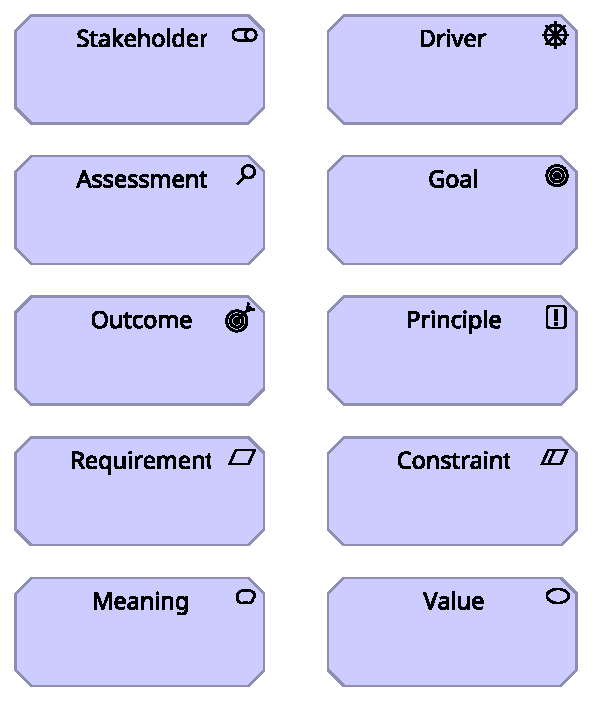
\includegraphics[height=0.7\textheight]{motivation-legend.pdf}
    \column{0.54\textwidth}
    \footnotesize
    \begin{itemize}
      \item \textbf{Stakeholder} -- pihak berkepentingan.
      \item \textbf{Driver} -- pendorong perubahan.
      \item \textbf{Assessment} -- penilaian kondisi.
      \item \textbf{Goal / Outcome} -- sasaran \& capaian.
      \item \textbf{Requirement / Constraint} -- syarat \& batas.
      \item \textbf{Principle} -- aturan penuntun.
      \item \textbf{Meaning / Value} -- makna \& manfaat.
    \end{itemize}
  \end{columns}
  \takeaway{Semua memakai bentuk oktagon ungu; ikon pojok membedakan jenisnya.}
\end{frame}

\begin{frame}{Membedakan Elemen Motivasi}
  \vspace{6pt}
  \begin{itemize}
    \item \textbf{Sasaran (goal):} keadaan akhir yang ingin dicapai, sebaiknya
          terukur.
    \item \textbf{Hasil (outcome):} capaian konkret yang menandai sasaran
          tercapai.
    \item \textbf{Kebutuhan (requirement):} hal yang harus dipenuhi sistem.
    \item \textbf{Kendala (constraint):} batas yang tidak dapat dilanggar.
    \item \textbf{Prinsip (principle):} aturan umum penuntun keputusan.
  \end{itemize}
  \takeaway{Memisahkan keempatnya mencegah pencampuran cita-cita, ukuran,
  kewajiban, dan batasan.}
\end{frame}

% ============================================================
\section{Studi Kasus: Model Motivasi}
\sectionframe{Studi Kasus: Model Motivasi}

\begin{frame}{Pemangku Kepentingan dan Concern}
  \vspace{2pt}
  \scriptsize
  \setlength{\extrarowheight}{2pt}
  \arrayrulecolor{black!65}\setlength{\arrayrulewidth}{0.4pt}
  \begin{tabularx}{\textwidth}{|p{0.28\textwidth}|X|}
    \hline
    \textbf{Pemangku Kepentingan} & \textbf{Concern Utama} \\
    \hline
    Pimpinan/Direksi & Biaya terkendali, peluncuran cepat, pertumbuhan UMKM. \\
    \hline
    Unit bisnis UMKM & Transfer instan 24/7 yang mudah dipakai dan dijual. \\
    \hline
    Divisi kepatuhan & APU-PPT, limit, jejak audit, SNAP BI, UU PDP (Undang-Undang Pelindungan Data Pribadi). \\
    \hline
    Tim teknologi & Integrasi aman ke BI-FAST dan core lama; keandalan. \\
    \hline
    Nasabah \& mitra & Perpindahan dana cepat, andal, transparan biayanya. \\
    \hline
    Regulator (Bank Indonesia; OJK, Otoritas Jasa Keuangan) & Kepatuhan standar, keamanan, perlindungan konsumen. \\
    \hline
  \end{tabularx}
\end{frame}

\begin{frame}{Pendorong $\rightarrow$ Asesmen $\rightarrow$ Sasaran}
  \vspace{2pt}
  \scriptsize
  \setlength{\extrarowheight}{2pt}
  \arrayrulecolor{black!65}\setlength{\arrayrulewidth}{0.4pt}
  \begin{tabularx}{\textwidth}{|p{0.24\textwidth}|X|X|}
    \hline
    \textbf{Pendorong} & \textbf{Asesmen Saat Ini} & \textbf{Sasaran/Hasil} \\
    \hline
    Ekspektasi transfer instan & Sebagian transfer batch (SKNBI, Sistem Kliring Nasional Bank Indonesia), manual. &
    Transfer real-time 24/7 lewat kanal dan API. \\
    \hline
    Persaingan fintech & UMKM beralih ke dompet digital. & Bank jadi pilihan
    rel transfer UMKM. \\
    \hline
    Kepatuhan SNAP BI / APU-PPT & BI-FAST belum jadi API terkelola; AML (\emph{anti-money laundering}) manual.
    & API patuh SNAP BI; penyaringan otomatis. \\
    \hline
    Efisiensi operasional & Rekonsiliasi manual, mahal, rawan salah. &
    Rekonsiliasi otomatis; biaya turun. \\
    \hline
  \end{tabularx}
  
  \vspace{5pt}
  \takeaway{Kebutuhan: wrapper BI-FAST, AML/limit otomatis, patuh SNAP BI.
  Kendala: anggaran, core lama, sertifikasi.}
\end{frame}

\begin{frame}{}
  \centering
  \vspace{1mm}
  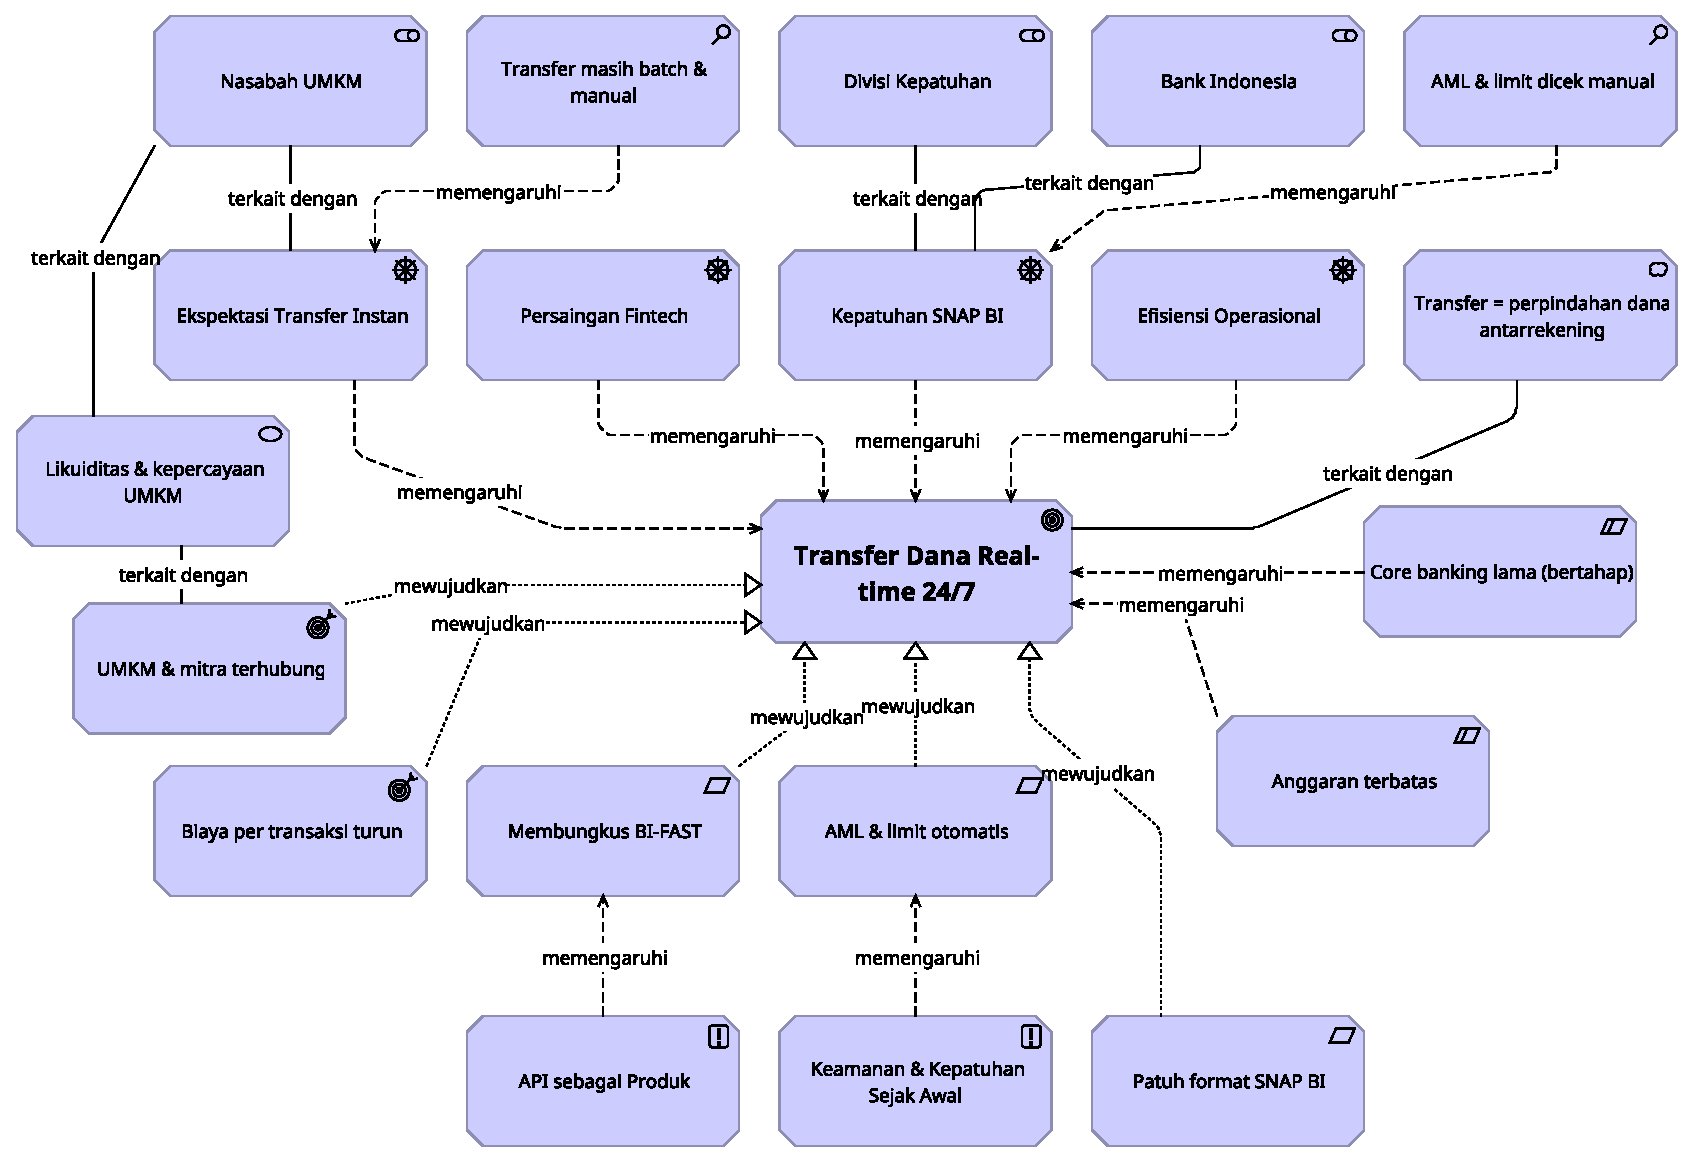
\includegraphics[height=.9\textheight]{motivation-transfer.pdf}\\
  {\scriptsize Model Motivasi ArchiMate dibangun dengan Archi.}
\end{frame}

\begin{frame}{Cara Membaca Diagram}
  \vspace{6pt}
  Tiga jenis hubungan menautkan elemen menjadi satu rantai argumentasi:
  \begin{itemize}
    \item \textbf{Asosiasi} -- konsep yang berkaitan erat (Nasabah UMKM
          $\sim$ ekspektasi; nilai $\sim$ penerima manfaat).
    \item \textbf{Pengaruh} -- mendorong/membatasi (persaingan mendorong
          sasaran; anggaran membatasi cara mewujudkannya).
    \item \textbf{Realisasi} -- membuat sasaran konkret (kebutuhan membungkus
          BI-FAST; hasil biaya turun).
  \end{itemize}
  \takeaway{Empat driver bertemu pada satu \textbf{sasaran pusat}; setiap
  kebutuhan dapat ditelusuri ke sasaran dan prinsip.}
\end{frame}

% ============================================================
\section{Dari Motivasi ke Masalah dan RQ}
\sectionframe{Dari Motivasi ke Masalah dan RQ}

\begin{frame}{Ketidakselarasan Utama}
  \vspace{8pt}
  \begin{enumerate}
    \item Sasaran transfer instan \emph{vs.} proses batch dan manual.
    \item Ambisi kemitraan \emph{vs.} ketiadaan API transfer terkelola.
    \item Tuntutan kepatuhan \emph{vs.} kontrol AML/limit manual.
    \item Sasaran efisiensi \emph{vs.} rekonsiliasi manual.
  \end{enumerate}
  \takeaway{Ketidakselarasan inilah bahan baku rumusan masalah.}
\end{frame}

\begin{frame}{Rumusan Masalah, RQ, dan Kontribusi}
  \vspace{4pt}
  \footnotesize
  \textbf{Rumusan masalah.} Sasaran transfer real-time bagi UMKM belum didukung
  rel perpindahan dana yang terkelola, patuh SNAP BI, dan terkendali risikonya.

  \vspace{4pt}
  \textbf{RQ.} Bagaimana pendekatan \emph{Enterprise Architecture} (EA) memakai
  TOGAF-lite (TOGAF: \emph{The Open Group Architecture Framework}) dan pemodelan
  motivasi ArchiMate untuk merumuskan arah arsitektur API Transfer Dana yang
  menyelaraskan kebutuhan UMKM, kepatuhan SNAP BI/UU PDP, dan kendala sistem
  inti?

  \vspace{4pt}
  \textbf{Kontribusi.} Model motivasi, daftar kebutuhan, dan prinsip yang
  realistis untuk rel transfer bank daerah; contoh penerapan pemodelan motivasi
  ArchiMate dan TOGAF-lite.
\end{frame}

% ============================================================
\section{Latihan dan Jembatan}
\sectionframe{Latihan dan Jembatan}

\begin{frame}{Latihan Terapan Individual}
  \vspace{8pt}
  \begin{itemize}
    \item \textbf{Latihan 3.1} -- Peta stakeholder dan driver untuk satu
          kapabilitas sasaran organisasi Anda.
    \item \textbf{Latihan 3.2} -- Sasaran, kebutuhan, kendala, dan prinsip.
    \item \textbf{Latihan 3.3} -- Draf rumusan masalah, RQ, dan kontribusi.
    \item \textbf{Latihan 3.4} -- Uji kelayakan terhadap target publikasi.
  \end{itemize}
  \takeaway{Semua latihan menjadi bahan langsung bagian Pendahuluan makalah.}
\end{frame}

\begin{frame}{Jembatan ke Bab Berikutnya}
  \vspace{8pt}
  \begin{itemize}
    \item Bab 4 naik ke \textbf{lapisan strategi}: \emph{course of action},
          kapabilitas, sumber daya, dan visi arsitektur.
    \item Keputusan strategis Bank Wanua: membangun \textbf{rel transfer lebih
          dahulu} sebelum layanan pembayaran lain.
    \item TOGAF-lite dipakai untuk menyusun visi, peta jalan, dan analisis
          kesenjangan; bibliografi awal mulai dibangun.
  \end{itemize}
  \takeaway{Motivasi yang jelas adalah kompas bagi strategi, bisnis, dan
  rancangan teknis berikutnya.}
\end{frame}

\begin{frame}{\hfill}
  \centering
  \Huge{\textbf{Terima kasih}}\\[8pt]
  \normalsize Pertanyaan \& diskusi
\end{frame}

\end{document}
